\capitulo{5}{Aspectos relevantes del desarrollo del proyecto}

En este apartado se van a relatar los aspectos más relevantes del desarrollo del proyecto, pasando de manera ordenada por todas las fases que fueron surgiendo durante dicho desarrollo.

\section{Proceso Inicial - Investigación, Comparativa y Elección}

En la etapa incial del proyecto se realizó una labor de investigación sobre diferentes herramientas y plataformas de corrección automática de ejercicios. En esta etapa fueron consideradas diferentes herramientas con el fin de obtener los conocimientos de partida necesarios y elegir una de ellas para su utilización dentro de nuestro proyecto. Estas herramientas han sido listadas y explicadas en el apartado \ref{OtrasHerramientas} \textit{Otras Herramientas Estudiadas} en el capítulo de \textit{Técnicas y Herramientas}. A continuación será explicada la aportación que estas herramientas dieron al proyecto y la razón por la que fueron descartadas:

\begin{itemize}
\item \textbf{CodeGrade:} Al tratarse de una plataforma independiente y completa, esta no fue considerada como una opción de uso dentro de nuestro proyecto, sin embargo, proporcionó información acerca del funcionamiento de plataformas de corrección automática de ejercicos en lenguajes de programación.

\item \textbf{CodingRooms:} De forma similar a CodeGrade, esta plataforma no fue estudiada con el propósito de ser usada dentro del proyecto, sino como fuente de información sobre la calificación automática de ejercicios.


\item \textbf{Otter-Grader:} Diversos problemas en la instalación y prueba de esta herramienta hicieron que Otter-Grader fuera descartada como herramienta de autograding pese a parecer en un primer momento una buena opción para nuestro proyecto.

\item \textbf{CS 41 Autograder:} La falta de documentación acerca de la instalación y uso de esta herramienta hizo que fuera descartada como autograder para nuestro proyecto.

\end{itemize}
Finalmente Nbgrader fue seleccionada como herramienta de autograding dentro de nuestro proyecto debido a su facilidad de instalación y uso intuitivo dentro de Jupyter Notebooks, el cual es considerado el entorno de ejecución de código Python más popular del momento.


\section{Desarrollo del Curso Introductorio a Python}
Uno de los objetivos principales del proyecto consistía en tener alojado dentro de nuestra plataforma un sencillo curso introductorio a Python, junto con sus respectivas tareas corregibles de forma automática, a disposición de los alumnos. Para ello se realizó una búsqueda de cursos introductorios a Python con el propósito de escoger uno como referencia para nuestro curso. Tras esta búsqueda el escogido fue el de "Python Para Todos" \cite{PythonParaTodos} de Raúl González Duque debido a la claridad y sencillez en sus explicaciones, además de aportar útiles ejemplos para su comprensión.

Una vez diseñado el contenido teórico de nuestro curso en Notebooks de Jupyte,r se diseñaron los conjuntos de ejercicios correspondientes a cada unidad de contenido adaptados a la herramienta de autograding seleccionada, Nbgrader.


\section{Jupyter Notebooks en Docker}
Debido a que una de las funcionalidades buscadas debía ser la creación de tareas por parte del profesor desde la propia plataforma, resultaba necesaria la ejecución de Jupyter Notebooks de forma remota junto con Nbgrader instalado en él. Por ello, tras varias pruebas realizadas, se logró la instalación de Jupyter dentro de un contenedor Docker y la ejecución remota de este gracias a la funcionalidad de mapeo de puertos que Docker ofrece.



\section{Desarrollo de la plataforma}
El proceso de desarrollo de la plataforma fue dividido en diversas fases: Creación del login inicial, creación de las tablas de la base de datos necesarias para el correcto funcionamiento futuro de la plataforma, desarrollo de las funcionalidades dirigidas a los alumnos, desarrollo de las funcionalidades dirigidas a los profesores, adición de estilos y landing, adición de funcionalidades extra y despliegue. A continuación entraremos en detalle dentro de cada una de ellas.

\subsection{Login inicial}
El proceso de creación del login de la plataforma fue la primera toma de contacto con Flask junto con sus herramientas Flask-Login y Flask-SQLAlchemy. Esta tarea no fue de gran dificultad pero nos presentó el primer reto de la plataforma: la distinción entre usuarios de tipo alumno o estudiante, y usuarios de tipo profesor. Este reto fue solucionado mediante un campo booleano dentro del modelo de usuario denominado ''is\_teacher'' campo que lograba la diferenciación entre tipos de usuarios.

\begin{figure}[h]
    \centering
    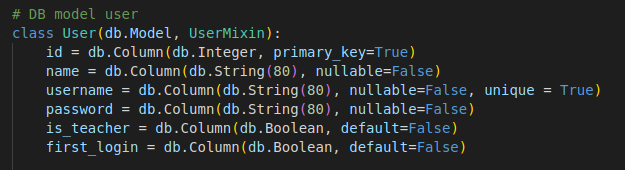
\includegraphics[scale=0.9]{img/imgs-memoria/UserModel.PNG}
    \caption{Modelo usuario}
\end{figure}

\subsection{Tablas de la base de datos}
Una vez obtenido un login funcional y como paso previo al desarrollo de las funcionalidades de la página, era necesaria la creación de las distintas tablas de base de datos las cuales nuestro futuro sistema dependería para funcionar, a excepción de la tabla usuarios la cual había sido requerida su implementación en el desarrollo del login. Esta taréa no fue de gran dificultad debido al fácil manejo que ofrece la herramienta SQLAlchemy y su utilización conjunta con Flask. 

La especificación concreta de tablas de la base de datos queda redactada en la sección \textit{C.2.Diseño de Datos} dentro del \textit{Anexo C: Especificación de diseño}.

\subsection{Funcionalidades para los alumnos}
Con las tablas necesarias para el funcionamiento de la plataforma ya creadas, el siguienta paso era la adición de todas las funcionalidades del alumno planeadas incialmente, las cuales consistían en: 
\begin{itemize}
\item Acceso a los cursos en los que el alumno está inscrito, junto con sus contenidos teóricos y tareas.
\item Entrega de las tareas resueltas y califición de forma automática.
\item Visualización de las calificaciones obtenidas en las tareas entregadas.
\item Cambio de contraseña.
\item Cierre de sesión.
\end{itemize}
Las anteriores funcionalidades descritas, a excepción de la entrega de tareas, fueron implementadas mediante funciones de Flask básicas. Sin embargo, para lograr la calificación automática de tareas tras la entrega de estas, fue necesaria la adaptación de la API pública de Nbgrader\cite{tool:NbgraderAPI} mediante una nueva clase dentro del proyecto denominada NbgraderManager, la cual sería completada posteriormente en el desarrollo de las funcionalidades para los profesores.

\subsection{Funcionalidades para los profesores}
Una vez añadidas las funcionalidades del alumno descritas en la sección anterior, llegaba el turno de los profesores. Estas funcionalidades iniciales eran las siguientes:
\begin{itemize}
\item Adición de cursos didáctivos y acceso a sus contenidos.
\item Creación de secciones de contenido dentro de un curso de forma directa (tarea creada previamente por el profesor de forma independiente).
\item Creación de secciones de contenido de forma indirecta (tarea creada desde la propia plataforma).
\item Consulta de calificaciones.
\item Inscripción y expulsión de alumnos en cursos.
\item Creación y eliminación de alumnos.
\item Cambio de contraseña.
\item Cierre de sesión.
\end{itemize}
Para las opciones de creación de secciones de contenido fue necesaria la adaptación de diversos métodos de la API de Nbgrader, completándose así la clase NbgraderManager mencionada con anterioridad. Adicionalmente, se adaptó el manejo de Jupyter Notebook dentro del código para hacer posible la edición de tareas desde la plataforma.

Debido a que nuestra plataforma no estaba orientada a contener usuarios de tipo administrador, en lo que respecta a la creación de nuevos alumnos se tomó la decisión de dejar esta tarea en manos de los profesores, quienes eligirían tanto nombre de usuario como contraseña para el alumno en cuestión. Con el fin de proteger la privacidad del alumno y darle a este la posibilidad de elegir su propia contraseña, cuando un alumno accede por primera vez a la plataforma con la contraseña escogida por el profesor, será direccionado de forma automática a la página de cambio de contraseña para que pueda escoger la contraseña de su cuenta personalmente, cambiando la dada incialmente por el profesor.
 
\subsection{Estilos y landing inicial}
Una vez completadas las funcionalidades inicialmente pensadas para profesores y alumnos, llegaba el momento de mejorar la estética de la plataforma, comenzando esta labor con la creación de un landing y, posteriormente, dando estilos al resto de vistas.

Los estilos del landing inicial y la página del login se dieron principalmente mediante CSS, a diferencia del resto de vistas las cuales recibieron sus estilos mediante la herramienta Bootstrap. Adicionalmente y con el objetivo de dar seguridad en la página frente a algunas acciones como el cierre de sesión, eliminación de alumnos o inscripción y baja de alumnos en cursos, fueron añadidas ventanas modales de confirmación de acciones mediante JavaScript.

Este proceso resultó un reto mayor de lo esperado dado que el presente Grado Universitado no profundiza demasiado en el manejo de estas herramientas. Por ello, fue necesario el estudio y práctica de estas herramientas hasta conseguir la adecuada soltura en su manejo.

\subsection{Adición de funcionalidades extra}
Tras finalizar la adición de estilos y con todas las funcionalidades previstas incialmente incluidas en la plataforma, surgió la necesidad de añadir nuevas opciones de funcionamiento debido a un mal diseño incial, que únicamente permitía la creación de cursos y secciones pero no su posterior eliminación. Junto a estas fueron añadidas otras funcionalidades orientadas al acceso a archivos relativos a las tareas y sus procesos de corrección automática:
\begin{itemize}
\item Eliminación de cursos existentes.
\item Eliminación de secciones de contenido de los cursos.
\item Descarga de los documentos tarea entregados por los alumnos.
\item Descarga de las tareas en versión profesor y alumno por parte de los profesores.
\item Posibilidad de publicación o cancelación de secciones aún no publicadas.
\item Descarga del estado actual de las tareas de las secciones aún no publicadas.
\item Descarga de documentos feedback de las tareas entregadas por parte de los alumnos.
\item Eliminación de calificaciones / entregas de tareas para permitir nuevos intentos.
\end{itemize}

La práctica en el manejo de Flask, Modales JS y adición de estilos conseguida durante el desarrollo de las funcionalidades previas hicieron de esta adición de nuevas funcionalidades una tarea mucho más sencilla en comparación con los retos a los que nos habíamos enfrentado con anterioridad.

\section{Despliegue}
Una vez finalizado el desarrollo de la plataforma y teniendo esta el funcionamiento esperado, llegaba el momento de su despliegue posibilitando el acceso al público a ella. Esto parecía que iba a resultar una tarea complicada y dilatada en el tiempo pero, gracias a la capa de servicios gratuita de Amazon Web Service (AWS), su realización fue más sencilla de lo esperado.

La profundización sobre el despliegue de la plataforma dentro de una instancia EC2 de AWS queda desarrollada en el \textit{Manual del Programador} incluido en el \textit{Anexo D: Documentación técnica de programación}.